Pour ce qui concerne les caps, la première étape a été de transformer à partir de la
formule de Black les prix qui leurs sont implicites, en sachant que leurs taux d'exercice,
les caps étant à la monnaie, correspondent aux taux swap. Cette fonction est implémentée
dans la méthode \verb+cap(T,+$\sigma$\verb+):cir.py+. Mathématiquement, on en trouve
l'expression dans \cite{brigo} à la p.~17.

On trouve alors les prix suivants reportés à la Table \ref{cap_table}.
\begin{table}
  \centering
  \caption{}
  \label{cap_table}
\begin{tabular}{rrr}
\toprule
 $T$ &         Prix cap &     $\sigma$ \\
\midrule
   1 & \num{0.000373}\$ & \num{0.6004} \\
   2 & \num{0.003607}\$ & \num{0.6317} \\
   3 & \num{0.012168}\$ & \num{0.5478} \\
   4 & \num{0.022158}\$ & \num{0.4862} \\
   5 & \num{0.031992}\$ & \num{0.4466} \\
   6 & \num{0.041089}\$ & \num{0.4134} \\
   7 & \num{0.051609}\$ & \num{0.4125} \\
   8 & \num{0.062394}\$ & \num{0.4125} \\
   9 & \num{0.065759}\$ & \num{0.3515} \\
  10 & \num{0.074157}\$ & \num{0.3428} \\
\bottomrule
\end{tabular}

\end{table}

Ces prix obtenus, il reste ensuite à calibrer le processus CIR++ afin de les
répliquer. Nous avons donc construit une fonction
\verb+cap_CIR(T,x0,k,+$\theta$\verb+,+$\sigma$\verb+):cir.py+ dont l'objectif est de
calculer le prix d'un cap à la monnaie selon une maturité et un ensemble de paramètres
CIR++, afin d'utiliser cette fonction dans une méthode de moindres carrés dont la sortie
devrait être semblable aux prix obtenus ci-haut.

Cette fonction est construite en faisant la somme de la valeur des caplets composant le
cap, puis en employant la relation caplet-put, suivi de la parité put-call
(\verb+ZBP(T,K,*+$\alpha$\verb+):cir.py+, pour enfin implémenter l'équation (3.78) de la
p.~103 de \cite{brigo} (\verb+ZBC(T,K,*+$\alpha$\verb+):cir.py+). Une telle implémentation
ne pose pas de problème particulier. Notons que dans le code, \verb+*+$\alpha$ réfère au
vecteur de paramètres CIR++.

Ceci étant dit, une fois l'algorithme de moindres carrés évalué (voir
\verb+load_cir_params():cir.py+), le processus de taux court en découlant peut être
particulièrement sujet à d'infâmes taux négatifs, pour peu qu'on n'y prenne garde. En
effet, soulignons d'une part que cet algorithme affiche une grande sensibilité aux valeurs
initiales données (reportées dans la Table \ref{cir_table}). Mais d'autre part, puisque
$\bm E r_t = f(0,t)$ et que la courbe forward tombe à des valeurs très proches de zéro
autour d'un an, ces taux négatifs à courte échéance ont été presqu'impossibles à
éviter. Pour éviter les taux négatifs à plus longue échéance, nous avons suivi les
conseils prodigués par \cite{brigo} p.~108, notamment en bornant le facteur $\theta$, qui
correspond à la limite asymptotique en distribution du processus CIR sous jacent au CIR++,
par un ordre de grandeur de $f(0,10)$ (voir Table \ref{cir_table}).

\begin{table}
  \centering
  \caption{}
  \label{cir_table}
  \begin{tabular}{lllll}
\toprule
{} & Paramètres initiaux & Borne inférieure & Borne supérieure &       Paramètres obtenus \\
\midrule
$x_0$    &        \num{0.0001} &        $-\infty$ &           $R(0)$ &  \num{7.29180968883e-09} \\
$\sigma$ &           \num{0.6} &        $-\infty$ &         $\infty$ &     \num{0.136728733551} \\
$\theta$ &          \num{0.01} &        $-\infty$ &    $1.25f(0,10)$ &    \num{0.0338220970132} \\
$k$      &          \num{0.08} &                0 &             0.15 &     \num{0.321782134839} \\
\bottomrule
\end{tabular}

\end{table}

Pour ce qui concerne la simulation du processus (voir
\verb+cir_process(T,+$\tau$,\verb+N,x0,k,+$\theta,\sigma$\verb+):cir.py+), elle ne pose pas non
plus de problème particulier; il s'agit essentiellement d'ajouter un paramètre de
correction $\phi(t)$ à un processus CIR régulier. Ce procesus a été simulé en employant
l'agorithme décrit dans \cite{glasserman} à la p.~124.

Les résultats sont reportés à la figure \ref{processes} où sont présentés un échantillon
de 25 trajectoires de taux court jusqu'à une échéance de 10 ans. On remarque notamment
qu'à courte échéance la plupart des trajectoires tombent sous 0, mais rapidement elles
remontent et sont bornées à des taux positifs. La seconde figure illustre la moyenne de
5000 trajectoires qui reproduit la courbe forward. On remarque qu'à plus longue échéance,
la moyenne tend à donner des valeurs supérieures au forward théorique. Ceci doit être dû
au fait que les taux ont une distribution chi carrée décentrée, et donc des moments
d'ordre 3 (asymétrie) et 4 (kurtose) importants; autrement dit, la moyenne empirique tend
lentement vers la moyenne théorique. 

\begin{figure}
  \centering
  \begin{subfigure}{0.3\paperwidth}
    \centering
    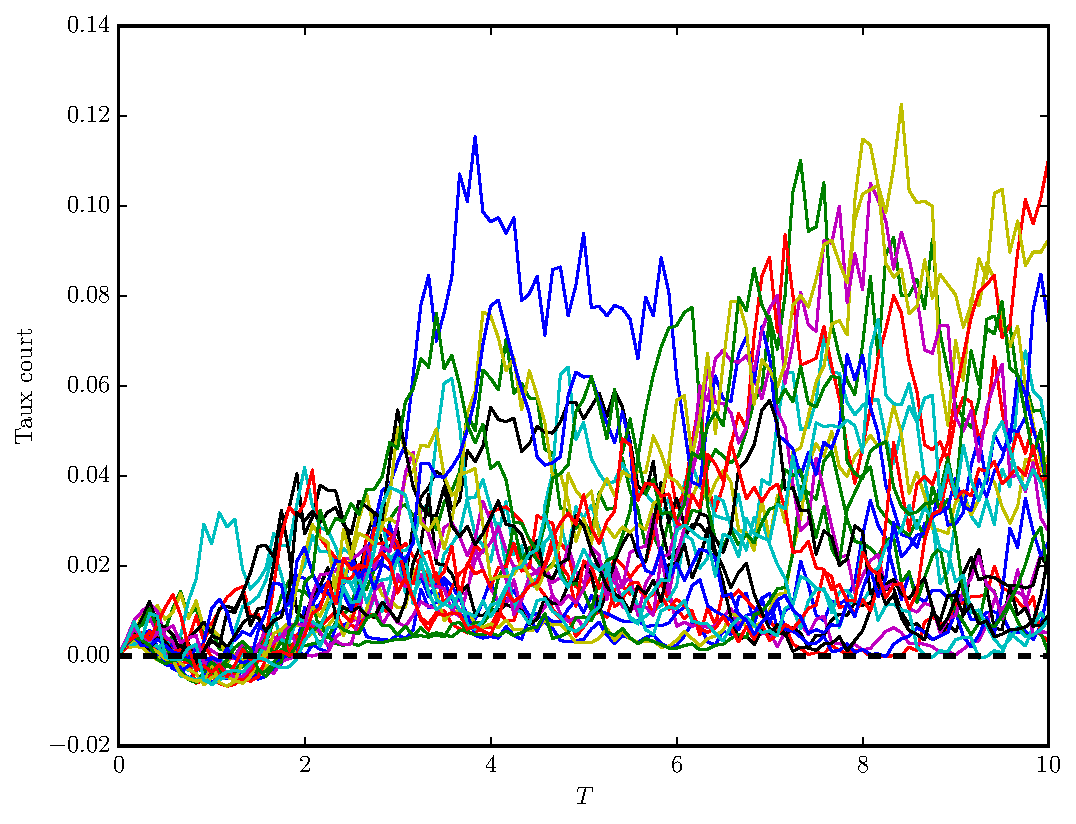
\includegraphics[width=0.3\paperwidth]{../fig/processes.pdf}
  \end{subfigure}
  ~
  \begin{subfigure}{0.3\paperwidth}
    \centering
    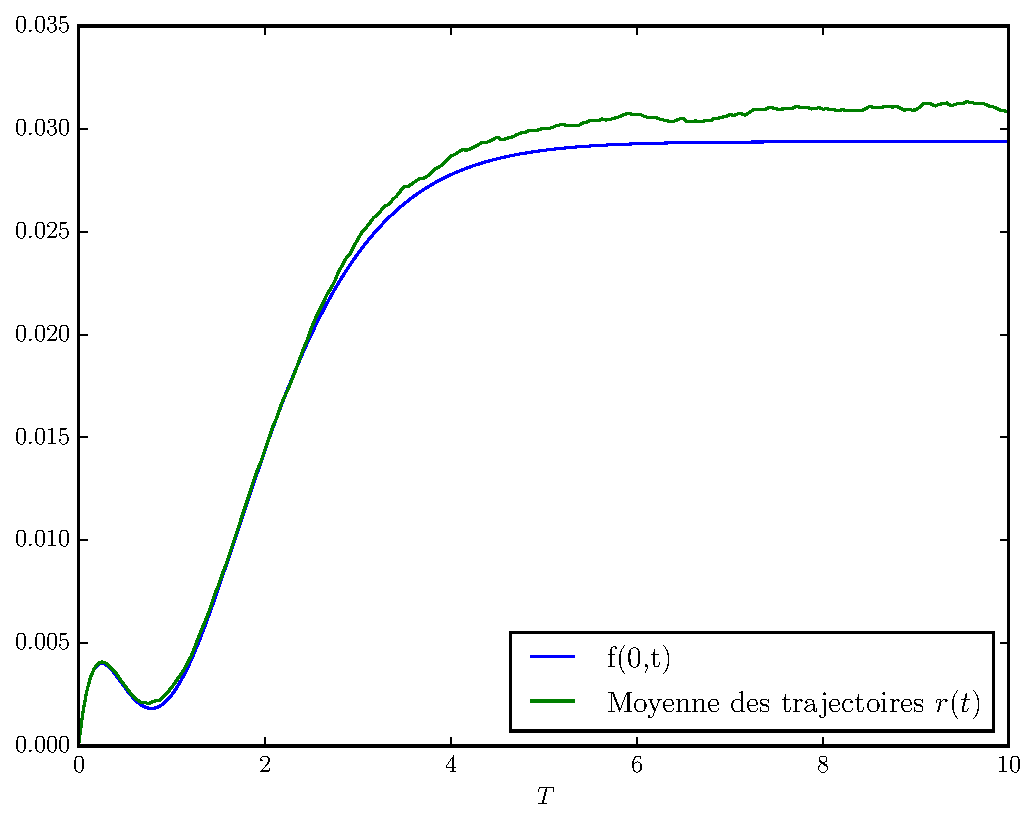
\includegraphics[width=0.3\paperwidth]{../fig/mean_p.pdf}
  \end{subfigure}
  \caption{}
  \label{processes}
\end{figure}

Finalement, la Figure \ref{capvol} reporte la valeur des caps empiriques par rapport à la
valeur des caps implicites au processus CIR++. On remarque que l'adéquation est
relativement bonne. Cependant, lorsqu'on inverse le prix des caps toujours avec la formule
de Black, pour de courtes échéances, on observe une différence assez importante, qui tend
à se réduire pour de plus faibles échéances. Ceci s'explique par le fait que pour de
courtes maturités, une très petite variation de prix entraînera une variation très
importante dans l'espace des volatilités.


\begin{figure}
  \centering
  \begin{subfigure}{0.3\paperwidth}
    \centering
    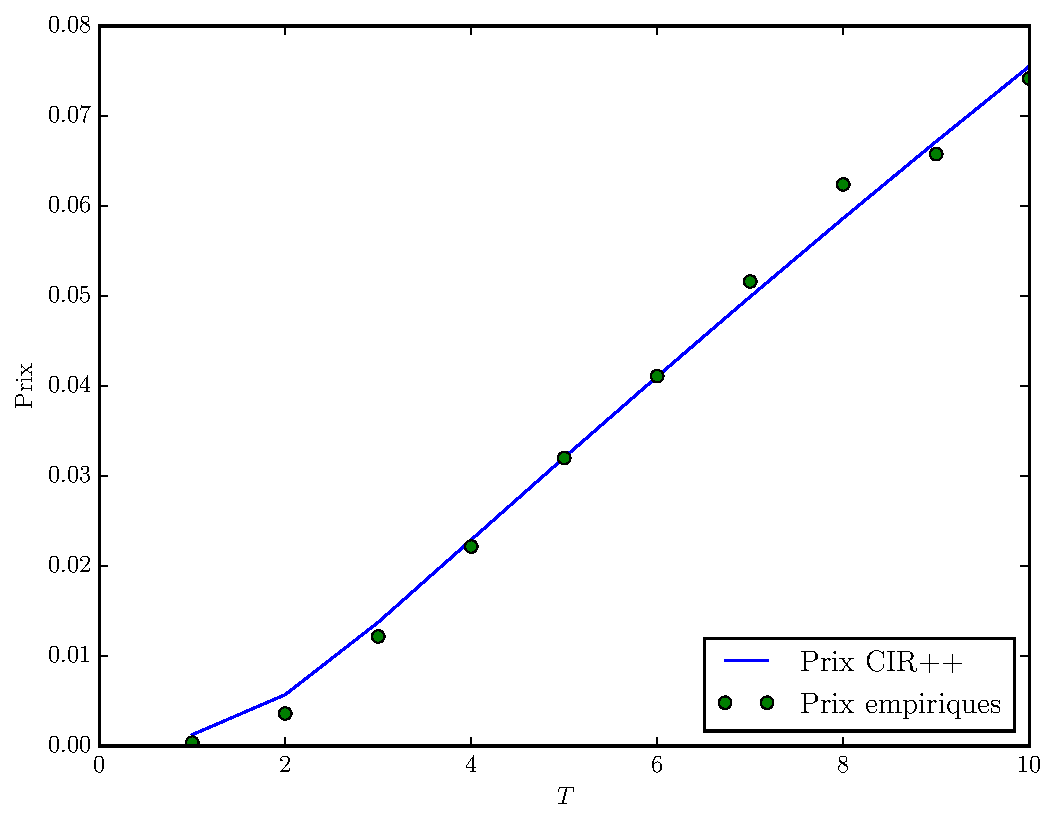
\includegraphics[width=0.3\paperwidth]{../fig/cap_price.pdf}
  \end{subfigure}
  ~
  \begin{subfigure}{0.3\paperwidth}
    \centering
    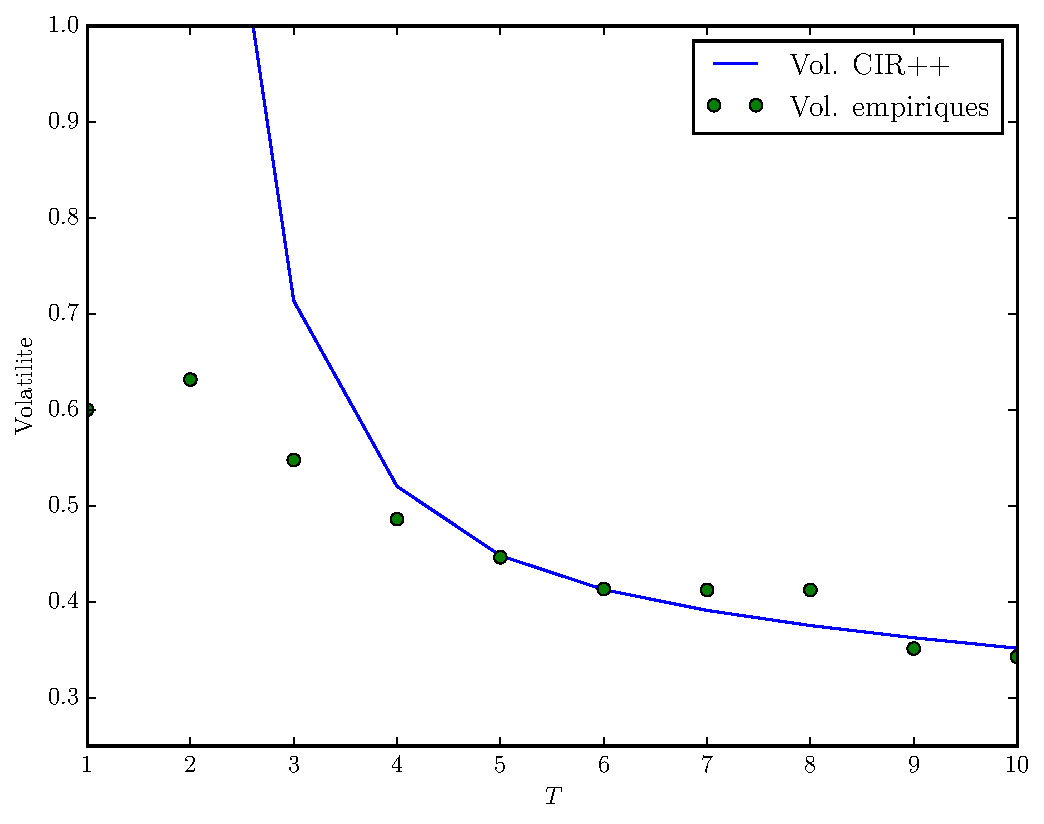
\includegraphics[width=0.3\paperwidth]{../fig/cap_vol.pdf}
  \end{subfigure}
  \caption{}
  \label{capvol}
\end{figure}

% Un algorithme de régions de confiance a de nouveau été employé. Notons par ailleurs que la
% méthode de résolution semblait particulièrement sensible aux données initiales. Ce fut en
% fait un véritable 


%%% Local Variables:
%%% mode: latex
%%% TeX-master: "rapport"
%%% End:
